We evaluate StarNet on two distinct surveys. First, we catalog the SDSS image of the Messier 2 (M2) globular cluster. 
Here, we are able to compare against an MCMC-based probabilistic cataloger, PCAT, as well as an algorithmic cataloging routine, DAOPHOT.
We evaluate the catalog quality by validating against data collected from 
the Hubble Space telescope

Then, we run StarNet on an image of our own Milky Way taken by the DECam survey,
and demonstrate the ability of StarNet to scale to large astronomical surveys.

\subsection{Results on the M2 globular cluster}
\label{sec:results_on_m2}

\begin{figure}[tb]
    \centering
    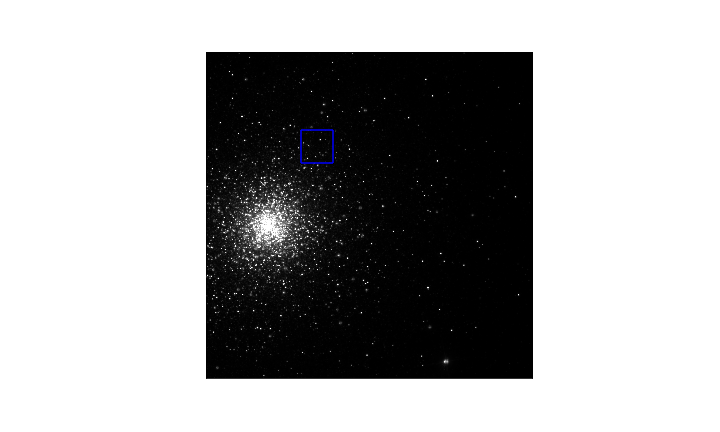
\includegraphics[width=0.7\textwidth]{figures/m2_results/m2_regions.png}
    \vspace{-1cm}
    \caption{The M2 globular cluster as imaged by SDSS. In blue is $100 \times 100$ subregion 
    cataloged by PCAT in \cite{Feder_2019}. }
    \label{fig:m2_region}
\end{figure}

The M2 globular cluster is a crowded starfield found in field 136 of camera column 2 in run 2583 of the SDSS survey. 
M2 was also imaged in the ACS Globular Cluster Survey~\citep{Sarajedini_2007}
using the Hubble Space telescope (HST),
which has greater resolution than the Sloan telescope.
The resolution of the HST wide-field channel is 0.05 arcseconds per pixel versus
0.4 arcseconds per pixel in SDSS \citep{hubble_about, sdss_about}.
For this image, the catalog from this Hubble survey (henceforth the ``HST catalog")
serves as ground truth for validating our results.

We first analyze the $100 \times 100$ pixel subimage of M2 that
\cite{Portillo_2017} and \cite{Feder_2019} analyzed with PCAT.
This subimage is located outside the heavily saturated core of the cluster (Figure~\ref{fig:m2_region}). 
However, in this subimage alone, the HST catalog contains 1114 stars with F606W-band magnitudes less than 22.
We include two bands in our model, the SDSS $r$-band and $i$-band.
The SDSS $r$-band and the Hubble F606W band are centered at roughly the same wavelength,
while the wavelength range of the Hubble F606W band is slightly broader.

We compare the cataloging accuracy of StarNet
to the two alternatives PCAT and DAOPHOT.
DAOPHOT is an algorithmic routine for detecting stars in crowded starfields
which does not use a generative model~\citep{stetson2987daophot}.
This software convolves the observed image with a Gaussian kernel and scans for peaks above a given threshold.
The DAOPHOT catalog of M2 was reported in \cite{An_2008_m2}.


% Both DAOPHOT and the Hubble survey produce a single catalog -- that is, a set of estimated stellar locations and fluxes -- with
% error bars nominally representing marginal uncertainties.
% In the context of probabilistic cataloging (StarNet and PCAT), the posterior
% defines a distribution over catalogs.
% Each sample from the (approximate) posterior returns a catalog, and each
% sampled catalog may have different cardinally.

To evaluate the three methods.
We filtered the ground truth HST catalog to stars with magnitudes smaller than 22.5 in the Hubble F606W band,
because none of the three methods were able to detect stars
with lower apparent brightness in the SDSS image.


Estimated catalogs are evaluated on three metrics: the true positive rate (TPR),
the positive predicted value (PPV), and the F1 score.
The TPR is the proportion of stars in the HST catalog matched with a star in the estimated catalog;
the PPV is the proportion of stars in the estimated catalog matched with a star in the HST catalog.
The F1 score summarizes the two metrics as the harmonic mean of the PPV and the TPR.

Like \cite{Portillo_2017} and \cite{Feder_2019}, a ``match" between an estimated star
and an HST star is defined as follows: (1) the estimated location and the HST location are within 0.5 SDSS pixels,
and (2) the estimated SDSS $r$-band flux and the HST F606W band flux are within half a magnitude.
% The slack in magnitude accounts for the fact that the wavelength range of the HST F606W band is slightly broader than the SDSS $r$-band (though they are centered at roughly the same wavelength).

In probabilistic cataloging (PCAT and StarNet), the posterior defines a distribution over catalogs.
For StarNet, the TPR, PPV, and F1 score were computed for the catalog corresponding to the mode of the variational distribution (henceforth, the StarNet catalog).
For PCAT, 300 catalogs were sampled using MCMC; the metrics were computed for each sampled catalog and averaged.

\begin{figure}[tb]
    \centering
    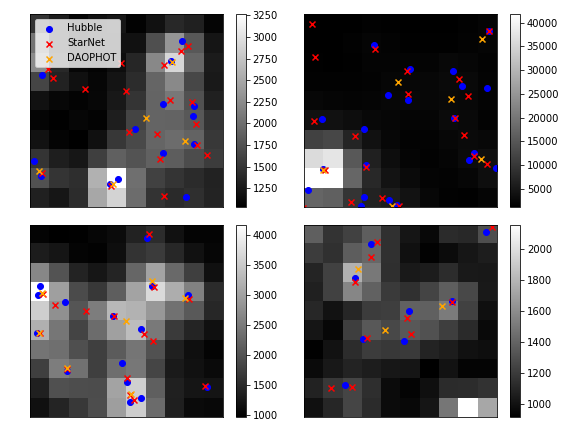
\includegraphics[width=0.49\textwidth]{figures/m2_results/example_subimages_starnet.png}
    \rulesep
    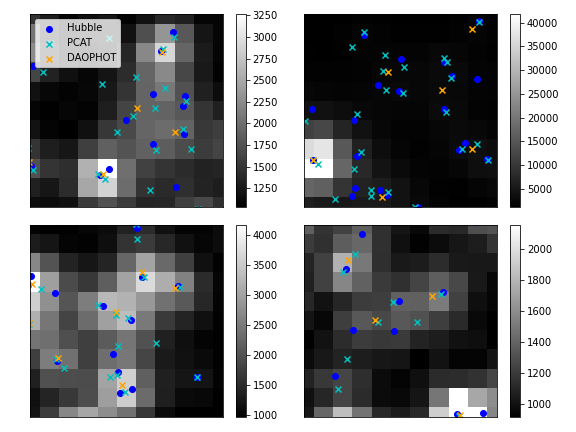
\includegraphics[width=0.49\textwidth]{figures/m2_results/example_subimages_pcat.png}
    % \vspace{-1cm}
    \caption{Estimated catalogs on four 10$\times$10 subimages from
    M2. Blue dots are stars from the HST catalog used as ground truth.
    StarNet, PCAT, and DAOPHOT estimated stars are shown as
    red, cyan, and orange crosses, respectively. }
    \label{fig:example_subimages}
\end{figure}

StarNet produced a catalog that outperforms DAOPHOT and PCAT in F1 score (Table~\ref{tab:summary_stats}).
Figure~\ref{fig:example_subimages} shows the StarNet catalog alongside PCAT, DAOPHOT, and HST catalogs.
DAOPHOT estimated less than half the number of stars when compared to the other methods.
It therefore had a large PPV but a small TPR.
The StarNet catalog had about the same TPR as PCAT while being ten percentage points higher in PPV.

Table~\ref{tab:summary_stats} also shows the number of stars inferred by each method.
There are 1114 stars in the HST catalog.
For probabilistic methods (StarNet and PCAT),
we display the mean number of stars under the approximate posterior, along with the 5-th and 95-th quantiles.
We compute the StarNet credible intervals by sampling from the variational posterior. 
Recall that on each tile, the variational posterior on the number of stars is a categorical random variable; 
to construct a distribution for the number of stars on the whole image, we first sample from the per-tile categorical distribution, then sum over all tiles. 
StarNet credible intervals were three times wider than the PCAT intervals
and closer to the ground truth.
The small PCAT credible intervals may be indicative of an MCMC sampler that failed to mix well.

% \begin{table}[!tb]
% \centering
% \caption{Performance metrics on M2.
% For probabilistic methods (StarNet and PCAT)
% the ``\#stars" column refers to the mean number of stars under the (approximate) posterior, while the right-most column displays the 5-th and 95-th percentiles under the posterior. }
% \label{tab:summary_stats}
% \begin{tabular}{l|ccc|cc}
% \toprule
%      Method &   TPR &   PPV &  F1 score &  \#stars & (q-5\%, q-95\%)\\
% \midrule
%     DAOPHOT &  0.20 &  0.63 &      0.30 &     295 & -- \\
%        PCAT &  0.56 &  0.40 &      0.47 &    1672 & (1664, 1680)\\
%  Sleep-only &  0.51 &  0.47 &      0.49 &    1292 & (1260, 1324)\\
%  Wake-sleep &  0.51 &  0.60 &      0.55 &     1014 & (987, 1041)\\
%      %Hubble &  1.00 &  1.00 &      1.00 &     1114 & -- %\\
% \bottomrule
% \end{tabular}
% \end{table}

\begin{table}[!tb]
\centering
\caption{Performance metrics on M2.
For probabilistic methods (StarNet and PCAT)
the ``\#stars" columns provide the mean along with the 5th and 95th percentiles
for the number of stars under the (approximate) posterior,
The number of stars in the Hubble catalog is 1114. }
\label{tab:summary_stats}
\begin{tabular}{l|ccc|cc}
\toprule
& & & & \multicolumn{2}{c}{\#Stars} \\
     Method &   TPR &   PPV &  F1 score &  mean & (q-5\%, q-95\%)\\
\midrule
    DAOPHOT &  0.20 &  0.65 &      0.31 &     357 & -- \\
       PCAT &  0.55 &  0.37 &      0.44 &    1672 & (1664, 1680)\\
 StarNet (our) &  0.53 &  0.48 &      \textbf{0.50} &    1462 & (1430, 1497)\\
\bottomrule
\end{tabular}
\end{table}


The improvement of StarNet over PCAT in PPV was most pronounced for dim stars (Figure~\ref{fig:summary_stats}).
The TPR for StarNet was uniformly better than DAOPHOT across almost all magnitudes.
Of all methods, StarNet best approximated the HST flux distribution (Figure~\ref{fig:luminosity_fun_m2}).
% PCAT overestimated the number of dim stars with magnitudes greater than 21.
% In contrast, DAOPHOT failed to find stars with magnitudes greater than $21$.

% (Figures~\ref{fig:m2_flux_estimation} and \ref{fig:luminosity_fun_m2}).

\begin{figure}[tb]
    \centering
    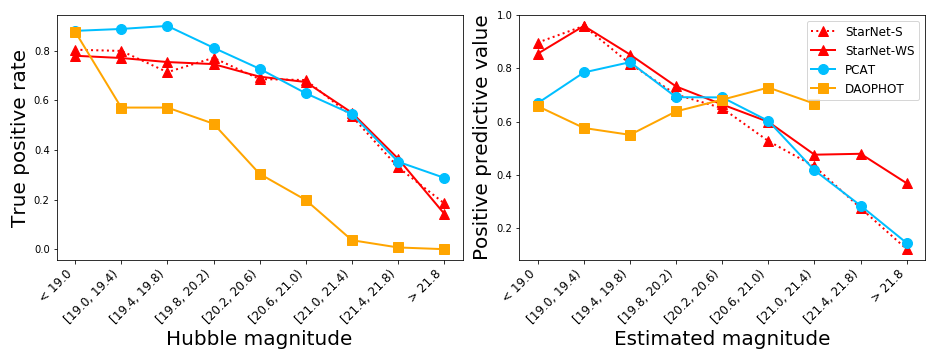
\includegraphics[width=0.99\textwidth]{figures/m2_results/summary_statistics_m2.png}
    \vspace{-0.4cm}
    \caption{True positive rate (left) and positive predicted value (right) of various cataloging
    procedures on M2, plotted against $r$-band magnitude.
    Smaller magnitudes correspond to brighter stars.
    }
    \label{fig:summary_stats}
\end{figure}

% \begin{figure}[tb]
%     \centering
%     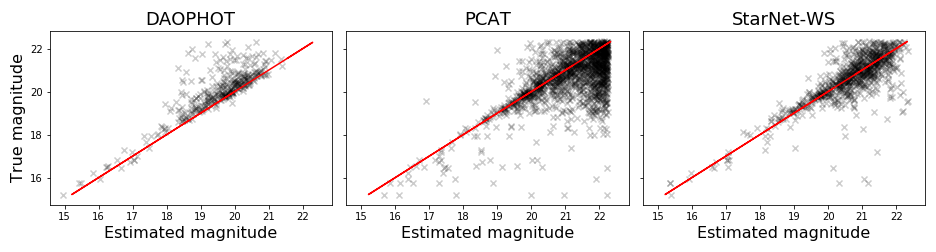
\includegraphics[width=0.99\textwidth]{figures/m2_results/m2_flux_estimation.png}
%     \caption{True versus estimated magnitudes on the $r$-band of M2.
%     Every estimated star was matched with the nearest Hubble star in L2 distance between locations.
%     Red line is the identity, $y=x$. }
%     \label{fig:m2_flux_estimation}
% \end{figure}

\begin{figure}[tb]
    \centering
    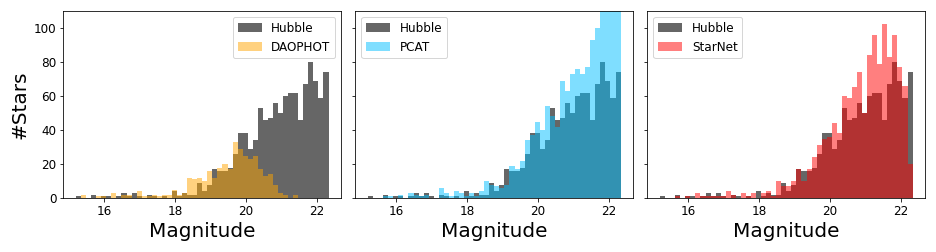
\includegraphics[width=0.99\textwidth]{figures/m2_results/luminosity_fun.png}
    \vspace{-0.4cm}
    \caption{Flux distributions for the $r$-band observations of M2.
    The flux distribution of the HST catalog in grey.
    Estimated distributions by DAOPHOT, PCAT, and StarNet catalogs overlaid.
    For PCAT, the flux distribution is from a single catalog sample. }
    \label{fig:luminosity_fun_m2}
\end{figure}


% \begin{figure}[tb]
%     \centering
%     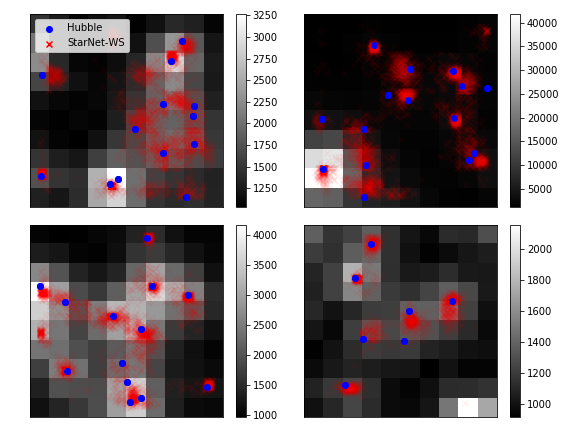
\includegraphics[width=0.49\textwidth]{figures/m2_results/example_subimages_samples_ws.png}
%     \rulesep
%     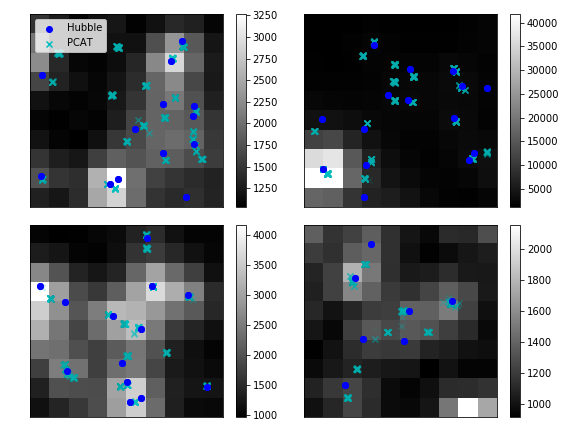
\includegraphics[width=0.49\textwidth]{figures/m2_results/example_subimages_samples_pcat.png}
%     \caption{Four 10$\times$10 subimages from
%     M2. Blue dots are stars from the HST catalog used as ground truth. (Left) Posterior samples from StarNet-WS and (right) posterior samples from the MCMC chain of PCAT. }
%     \label{fig:example_subimages_sampled}
% \end{figure}

% StarNet-WS returns a well-defined distribution over the set of all catalogs
% and is thus able to capture uncertainties in catalog construction.
% Samples from the StarNet-WS variational distribution are compared with samples from PCAT in Figure~\ref{fig:example_subimages_sampled}.
To examine the uncertainty calibration of StarNet, we evaluated the approximate posterior
conditional on the true number of stars in the HST catalog.
Then, each star in the StarNet catalog was matched with exactly one Hubble star by finding the permutation of Hubble stars that had the largest log-likelihood under our variational distribution $q_\eta$.
For each star, we computed the z-score $(y - \hat \mu) / \hat \sigma$, where $y$ is the HST log-flux or
logit-location; $\hat \mu$ and $\hat\sigma$ are the mean and the standard deviation, respectively, of the Gaussian variational distribution for the log-flux or logit-location.
% If the uncertainties were perfectly calibrated, the distribution of these z-scores would be a standard Gaussian.
The empirical z-score distributions are close to a standard Gaussian with some discrepancy in the tails and some evidence of skewness, suggesting the uncertainties are well-estimated (Figure~\ref{fig:z-score_calibration}).

\begin{figure}[tb]
    \centering
    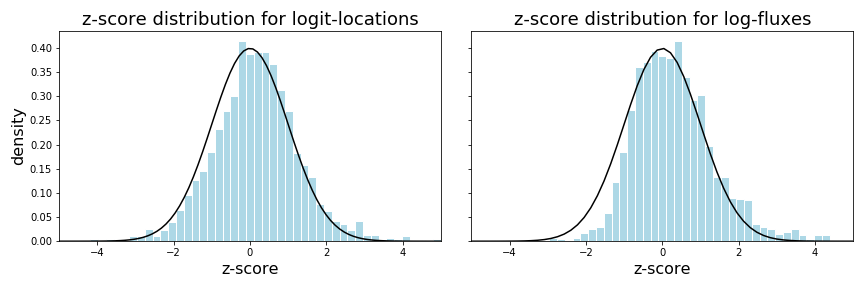
\includegraphics[width=0.99\textwidth]{figures/m2_results/zscore_calibration.png}
    \vspace{-0.5cm}
    \caption{The empirical distribution of z-scores for logit-locations (left) and log-fluxes (right) under the StarNet variational posterior.
}
    \label{fig:z-score_calibration}
\end{figure}

Finally, we catalog the entire M2 globular cluster, 
contained in a $1000 \times 1000$-pixel image (Figure~\ref{fig:m2_region}). We produce a color-magnitude diagram on this entire region. 
Restricting to only a $100\times100$ subimage 
does not reveal the second cluster of red (TODO)
stars that appear in the Hubble catalog. 
This cluster becomes salient after we filter to
high-confidence stars in the catalog, defined as stars with posterior standard deviation on the flux less than one. 

\begin{figure}[tb]
    \centering
    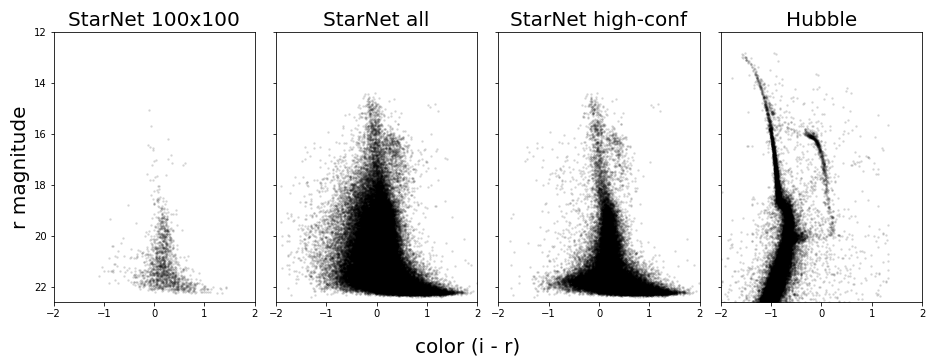
\includegraphics[width=0.99\textwidth]{figures/m2_results/m2_cmd.png}
    \vspace{-0.5cm}
    \caption{Color-magnitude diagrams from StarNet and Hubble. From left the right: color-magnitude diagram constructed from the same $100\times100$ subimage considered by PCAT; 
    the StarNet catalog constructed from the entire $1000 \times 1000$ image of M2; 
    the StarNet catalog then filtered to stars with posterior standard deviation on the flux less than one; the Hubble catalog. 
}
    \label{fig:m2_cmd}
\end{figure}

\subsubsection{Runtime}
\label{sec:runtime}
We ran SGD to minimize the expected forward KL
for 400 epochs; at each epoch, 200 images were sampled from the generative model.
Optimization was done with Adam~\citep{kingma2014adam}.
On a single NVIDIA GeForce RTX 2080 Ti GPU,
this fitting proceudre took about 50 minutes.

After fitting the model and variational posterior,
calculating the approximate posterior
(that is, producing the distributional parameters of the variational approximation) for the $100 \times 100$ pixel image of M2 took $30$ milliseconds.
By comparison, the reported runtime of PCAT, which uses MCMC, is 30 minutes on the same $100 \times 100$ pixel image~\citep{Feder_2019}.
Hence, after the initial fit, StarNet provided nearly a $10^5$-fold speed increase.

The speed at inference time (which excludes training time) gives StarNet the scaling characteristics necessary for processing large astronomical surveys.
A single SDSS image is $1489 \times 2048$ pixels.
Based on the reported 30-minute runtime of PCAT for a $100\times100$ pixel subimage, we project that
the runtime to process the full image would be $30\text{ min} \times 14 \times 20 = 8400$ minutes, or almost six days.
The SDSS survey consists of nearly one million images. Scaling PCAT to the entire SDSS survey would be infeasible.
The upcoming LSST survey will be 300 times larger than SDSS.

On the other hand, StarNet only incurs a one-time fitting cost.
After this initial fit,
producing a catalog with the full $1489 \times 2048$ pixel image requires
$30\text{ msec} \times 14 \times 20 = 8.4$ seconds. In practice,
inference can be made even faster by batching the image tiles to run in parallel on a GPU.

In the next subsection, we demonstrate the scaling characteristics on a frame from
the DECAPS survey.

% Figure~\ref{fig:cmd_m2} displays the estimated color-magnitude diagrams. While the Hubble F606W-band corresponds roughly to the SDSS $r$-band, there is no such correspondence for the SDSS $i$-band. Thus, using the Hubble locations, we estimated the $i$-band fluxes using maximum likelihood: letting $x^{(i)}$ be the SDSS image in the $i$-band, $N_H$ the number of stars in the Hubble catalog and $\ell_H$ their locations, solve
% \begin{align}
%   f^{(i)}_H = \argmax_{f\in\mathbb{R}^{N_H}} \log p(x^{(i)} | N_H, \ell_H, f)
%   \label{eq:optim_iband_flux},
% \end{align}
% where the log likelihood is given by the generative model from Section~\ref{sec:gen_model}.
% The estimated $i$-band fluxes and the reported Hubble F606W-band fluxes $f_H^{(r)}$ define the ``true" colors, $2.5\log(f_H^{(i)}/f_H^{(r)})$.
% In the color magnitude diagram, DAOPHOT did not capture the full spectrum of colors; of all three methods, PCAT best captured the color spectrum. All three methods however, were able to capture the arm thing (TODO there is a name for this ... main sequence turnoff?) that branches off at low magnitudes.

% \begin{figure}[ht]
%     \centering
%     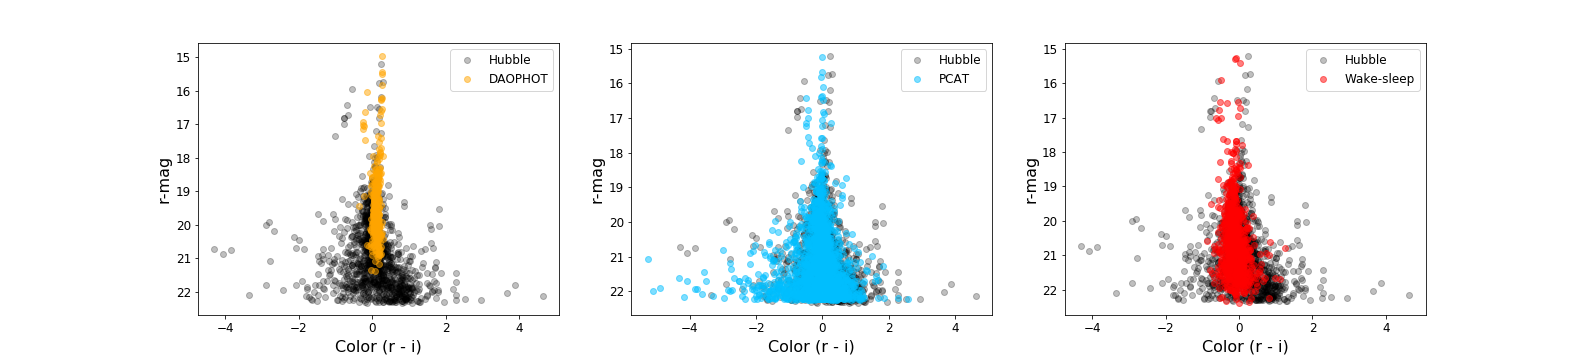
\includegraphics[width=0.99\textwidth]{figures/cmd.png}
%     \caption{Color magnitude diagrams on M2. }
%     \label{fig:cmd_m2}
% \end{figure}



% Figure~\ref{fig:loglik_table} displays the log-likelihood under the default SDSS estimates of the PSF and background compared with the estimates found using wake-sleep.
% The wake-sleep estimates improved the log-likelihood.
% We also compared against the ``Hubble estimate" of the background and PSF, obtained by minimizing $- \log p_\phi(x | N_{H}, \ell_{H}, f_{H})$ for $\phi$ directly.

% The results suggest that the primary source of model misfit is the background. A significant increase in log-likelihood occurred by switching from the SDSS background to the Hubble-estimated background.
% But even using the Hubble-estimated background, switching from the SDSS PSF to our wake-sleep PSF improves the log-likelihood.

% \begin{figure}[ht]
%     \centering
%     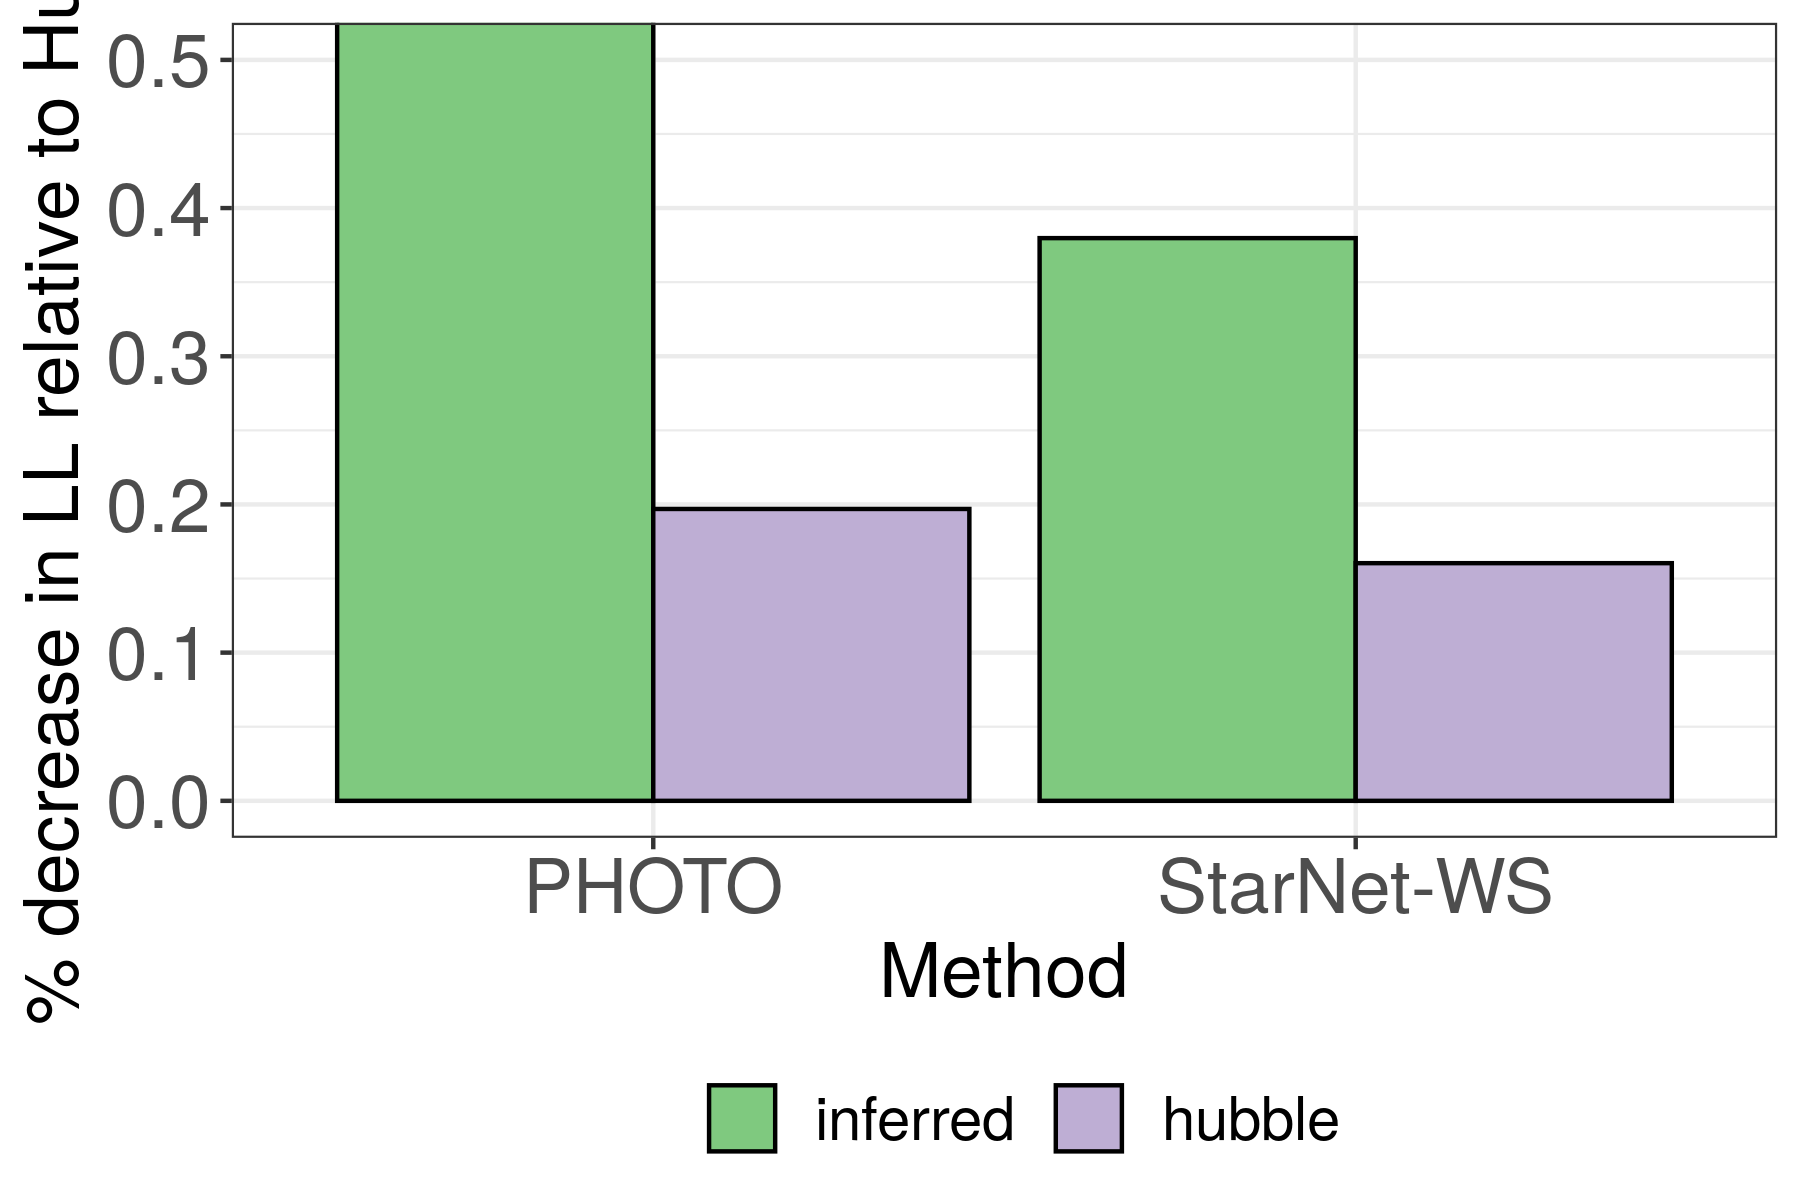
\includegraphics[width=0.6\textwidth]{figures/loglik_table.png}
%     \caption{Percent decrease in log-likelihood relative to the Hubble estimate of the PSF and background.
%     For each method, we evaluate the log-likelihood where the both PSF
%     and background are estimated (green);
%     we also show results where only the PSF is estimated (purple).
%     }
%     \label{fig:loglik_table}
% \end{figure}

% \input{tables/chi_sq_stats.txt}
% \caption{
% Negative log-likelihood for SDSS, wake-sleep, and Hubble estimated model parameters. In the right column, we fix the background to the Hubble estimate, and examine negative log-likelihood as the PSF varies.}

% The StarNet-based PSF did not differ from the SDSS PSF significantly. The greatest change was in the $r$-band PSF, where the SDSS PSF was most different from the Hubble-estimated PSF.

% \begin{figure}[ht]
%     \centering
%     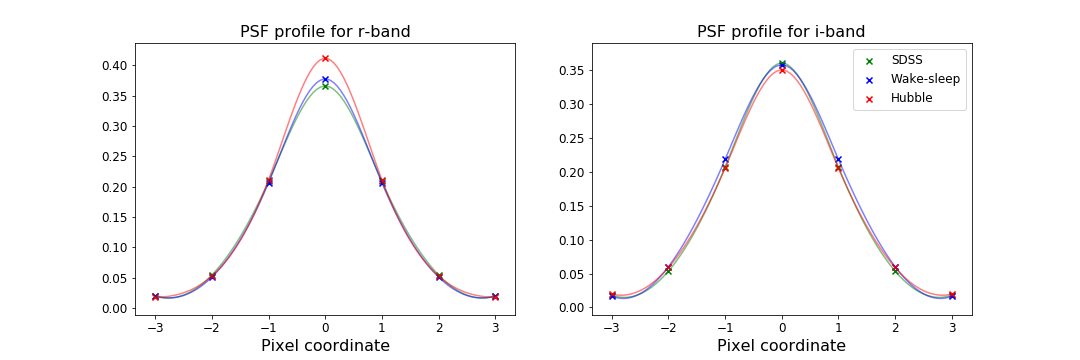
\includegraphics[width=0.99\textwidth]{figures/psf_profiles.png}
%     \caption{Estimated versus true PSF profiles on M2. The Hubble PSF was
%     obtained by optimizing the likelihood conditioned on locations and fluxes
%     from the Hubble catalog. TODO: this image is not that informative, I think I'll remove this. }
%     \label{fig:psf_profiles}
% \end{figure}


% \multicolumn{1}{p{5cm}}{\raggedleft Neg. loglik \\ (with Hubble back.)}
% \caption{
% Chi-squared statistics for SDSS, wake-sleep, and Hubble estimated model parameters.
% The chi-squared statistic is defined as
% $\sum_{bij}\frac{([\text{obs.image}]_{bij} - [\text{recon.image}]_{bij})^2}{[\text{recon.image}]_{bij}}$.
% In the middle column, ``model parameters" refer to both background and PSF.
% In the right column, we fix the background to the Hubble estimate, and examine
% chi-squared statistics as the PSF varies.}
